\documentclass{VUMIFPSkursinis}
\usepackage{algorithmicx}
\usepackage{algorithm}
\usepackage{algpseudocode}
\usepackage{amsfonts}
\usepackage{amsmath}
\usepackage{bm}
\usepackage{caption}
\usepackage{color}
\usepackage{float}
\usepackage{graphicx}
\usepackage{listings}
\usepackage{subfig}
\usepackage{wrapfig}

% Titulinio aprašas
\university{Vilniaus universitetas}
\faculty{Matematikos ir informatikos fakultetas}
\department{Programų sistemų katedra}
\papertype{Kursinis darbas}
\title{Krepšinio taisyklių pažeidimo aptikimas}
\titleineng{Recognizing Violations of Basketball Rules using Computer Vision}
\status{3 kurso 6 grupės studentas}
\author{Lukas Cedronas}
% \secondauthor{Vardonis Pavardonis}   % Pridėti antrą autorių
\supervisor{partn. prof. dr. Vytautas Ašeris}
\date{Vilnius – \the\year}

% Nustatymai
% \setmainfont{Palemonas}   % Pakeisti teksto šriftą į Palemonas (turi būti įdiegtas sistemoje)
\bibliography{bibliografija}

\begin{document}
\maketitle

\tableofcontents

\sectionnonum{Įvadas}
Krepšinio dinamiškumas, intensyvumas ir populiarumas lemia tai, jog teisėjų priimami sprendimai gali būti šališki \cite{ProfitableBias} arba, dėl tokių faktorių kaip nuovargis, prastai pagrįsti \cite{MissedCalls}. Norint išvengti žmogiškųjų klaidų ir teisėjavimą padaryti objektyvesniu, į pagalbą galima pasitelkti kompiuterines technologijas. Technologijos, skirtos žaidimo įrašymui realiu laiku ir prieigai prie nufilmuotos medžiagos žaidimo metu teisėjų naudojama jau nuo seno, tačiau sritis, kurioje krepšinis dar nėra pažengęs, bet iš kurios galėtų gauti nemažai naudos – kompiuterinė rega (\textit{angl.} computer vision). Pasitelkus priemones, skirtas vaizdo apdorojimui, analizei ir automatizuotam sprendimų priėmimui galima iki tam tikro laipsnio teisėjavimo naštą perkelti kompiuteriui. Kompiuterio pagalba sporte ar sporto teisėjavime nėra naujiena – technologijų sėkmę gali paliudyti  2018 m. FIFA pasaulio čempionate naudotas Video Assistant Referee, peržiūrintis ir įvertinantis teisėjo padarytą nuosprendį. Tačiau nepaisant to, ši sritis nėra pakankamai pažengusi, kad visiškai pakeistų teisėjus. Bet kokiai programinei įrangai išanalizuoti vaizdo įrašą ir prieiti prie teisingo sprendimo trukdo tokie faktoriai kaip vaizdo kokybė, pasirinktas kameros kampas, judančių objektų susiliejimas, žaidėjų bei kamuolio spalvų panašumas, objektų smulkumas. Tad siekiant išbandyti pačio atpažinimo algoritmo efektyvumą kiek galima labiau atsiribojant nuo techninių kliūčių, šiame darbe bus naudojama vaizdinė medžiaga, kur:
\begin{itemize}
 \item Tarp fono, žaidėjo ir kamuolio turi būti kiek galima didesnis kontrastas.
 \item Kamuolio spalva – ryški, aukštas sodrumas (\textit{angl.} saturation).
 \item Fonas – šviesus, jame – kiek galima mažiau triukšmo (atpažinimui nereikalingų objektų).
 \item Žaidėjas su kamuoliu užima kiek įmanoma didesnį plotą visame kadre (tačiau vis dar privalo matytis kojos ir ranka).
 \item Kamera pastatyta prie žemės (tam, kad kuo geriau matytųsi, kaip ant paviršiaus dedama koja).
 \item Žaidėjas yra vienas.
 \item Žaidėjas dėvi ryškius batus ir pirštines.
\end{itemize}

Darbe bus išanalizuoti probleminiai faktoriai, sukeliantys trukdžių vaizdo atpažinime, pasirinktos metodikos, padedančios atpažinti kamuolio poziciją rankų atžvilgiu bei žingsnius, bei pritaikytas algoritmas atpažinti, kada pažeista žingsnių taisyklė. Darbo tikslas – sukurti programinę įrangą, gebančią atpažinti žingsnių taisyklės pažeidimą (šiame darbe bus remiamasi NBA taisyklėmis). Darbo uždaviniai:
\begin{itemize}
 \item Sukurti žingsnių bei kamuolio mušimo atpažinimo algoritmą.
 \item Remiantis skaitmeniniu vaizdo apdorojimo technologijomis algoritmą įgyvendinti.
 \item Įvertinti įgyvendintos programos efektyvumą su vaizdo medžiaga.
\end{itemize}

\section{Naudoti įrankiai ir metodai}
Šiam darbui atlikti pasirinkta Python programavimo kalba. Dėl Python paprastumo ir duomenų analizės specialistų polinkio naudoti šią kalbą internete gausu straipsnių ir kitų išteklių būtent šiai kalbai. Python leidžia susifokusuoti į aukšto lygmens abstrakcijas, kas labai praverčia kompiuterinėje regoje analizuojant ir darant operacijas su paveikslėliais, vaizdo medžiaga ir panašiai. Be to, kadangi Python yra interpretuojama programavimo kalba – jos nereikia kompiliuoti – atsiranda galimybė programuoti interaktyviai, t.y. greitai išgauti rezultatus iš įvairių skaičiavimų nevykdant iš naujo jau parašytos programos. 

Kompiuterinės regos algoritmų įgyvendinimui nagrinėtos dvi bibliotekos: SimpleCV \cite{SimpleCV} ir OpenCV \cite{OpenCV}. OpenCV – plačiai naudojama kompiuterinės regos užduotims spręsti skirta biblioteka, kuri yra nemokama. OpenCV parašyta C++ kalba, tačiau galima naudoti OpenCV su  Python apvalku ant C++ rašyto pagrindo. Taip pasiekiamas artimas C++ efektyvumas kartu su Python kalbos paprastumu.
SimpleCV – panaši biblioteka į OpenCV, tačiau dar labiau abstrahuota, fokusas į naudojamo paprastumą, prieinamumą pradedantiesiems. Dėl medžiagos gausos ir didesnių galimybių sukurti efektyvų algoritmą nuspręsta naudoti OpenCV.

Vaizdo medžiagai išgauti naudojama Xiaomi Redmi 5 Plus kamera, gebanti filmuoti 1080p, 60 kadrų per sekundę greičiu. 
\section{Pirminis vaizdo apdorojimas}
\subsection{Kompiuterinės regos algoritmai dominančių regionų išskyrimui}
Pirmiausia vaizdas yra apdorojamas, siekiant išgauti objektus, kuriems vėliau bus pritaikomas algoritmas. Šiame darbe analizuojami svarbiausi objektai yra trys: kamuolys, žaidėjo rankos ir pėdos. Tad programą galima išskirti į dvi dalis: pirmoji – naudojantis kompiuterinės regos algoritmais išgauti šiuos tris objektus ir sąveikas tarp jų, ir antroji – su gauta informacija atlikti žingsnius, aprašytus taisyklės pažeidimo algoritme. 

Galima pamanyti, jog užtenka atrasti apvalų objektą ir teigti, jog tai – kamuolys, tačiau reikia atsižvelgti į tai, kad: 
\begin{enumerate}
\item Negalima garantuoti, kad kamuolys yra vienintelis apvalus objektas kadre. Pavyzdžiui, į kadrą gali patekti žaidėjo galva, arba pėda gali būti pastatyta taip, jog algoritmas ją irgi palaikys apvaliu objektu. 
\item Net jei ir užtikriname, kad kamuolys – vienintelis apvalus objektas kadre, judėdamas jis tampa nebe toks apvalus. Jei kameros kokybė prastesnė, greitai judantis objektas gali tapti išsiliejęs ir ištemptas.
\end{enumerate}
\subsection{Segmentavimas}
Aukščiau išvardintų problemų sprendimui pasirinktas segmentavimo pagal spalvą metodas. Segmentavimas – procesas, kai vaizdas yra suskirstomas į nesikertančius regionus \cite{ImageSegmTech}. Tad segmentuojant pagal spalvą išskiriamas regionas, atitinkantis kamuolio vietą kadre, su prielaida, kad kamuolys bus kitokios, iš anksto apibrėžtos spalvos, negu bet kas kitas kadre. Šitaip programa galės nesunkiai išskirti kamuolį kaip atskirą objektą. 

Jei kamuolio spalva nėra pakankamai ryški ir išsiskirianti iš fono, minėtu metodu atpažinti kamuolį darosi sunku, todėl kamuolio spalva turi būti kiek galima sodresnė. Taip pat naudojamas HSV modelis, kuris padeda dalinai išspręsti šią problemą \cite{StaloTenisas}: pasinaudojus HSV modeliu, atpažinti kamuolį darosi lengviau, net jei kinta apšvietimas, kadangi spalva išlieka ta pati, keičiasi tik sodrumas kartu su šviesumu. Tačiau reikia atkreipti dėmesį, jog OpenCV naudojama spalvos skalė skiriasi nuo įprastos. Spalvos atspalvis (\textit{angl.} hue) išreiškiamas laipsniais nuo 0 iki 360, tačiau OpenCV kiekvienai reikšmei naudoja 8 bitų dydžio char reprezentaciją, todėl galimų reikšmių intervalas yra [0; 255]. Tad būtina atspalvio reikšmes normalizuoti (t.y. padalinti iš dviejų), prieš jas panaudojant OpenCV kontekste. Šiame darbe minint HSV reikšmes atspalviui bus naudojamas standartinis laipsnių modelis.

Taisyklės pažeidimo algoritmui reikia žinoti, kada kamuolys yra rankoje. Tačiau vykdant spalvos segmentavimą išskirti tik ranką yra beveik neįmanoma, jei rankos spalva sutampa su kitų elementų, esančių kadre, spalva – pavyzdžiui, žaidėjo odos. Tokiu atveju išskirti ranką kaip objektą yra keletas būdų – pavyzdžiui, Haar kaskadų metodas, paremtas kompiuterio mokymo principais: su pozityviais paveikslėliais (šiuo atveju tai būtų paveikslėlis, kuriame pavaizduota ranka) ir negatyviais (tai paveikslėliai, kurie nėra ranka) sukuriama atpažinimo formulė \cite{HaarCascades}.  Tačiau toks rankų atpažinimo metodas gana sudėtingas ir lėtas, todėl nuspręsta imtis kitos išeities – užsidėti pirštinę, kurios spalva būtų unikali visame kadre. Spalva pasirinkta geltona, jos atspalvio kodas svyruoja nuo 96 iki 112. Pasirinkus platesnį intervalą pradedami segmentuoti šalutiniai objektai, siauresnį - rankos regione atsiranda dėmės, kadangi ne visos spalvos būna rastos. Segmentavimo rezultatai matyti \ref{imgs:rank} paveikslėlyje. Po segmentavimo atsirado šiek tiek triukšmo, kuris bus pašalintas atliekant eroziją. Tokie patys principai pritaikomi ir pėdų (batų) bei kamuolio radimui.
\begin{figure}[H]
	\centering
	
\includegraphics[scale=1]{imgs/rank}
	\caption{Rankos prieš ir po segmentavimo.}
	\label{imgs:rank}
\end{figure}

\subsection{Morfologinės transformacijos}
Po segmentavimo išskirtas objektas gali turėti triukšmo (t.y. nereikalingų dėmių, smulkių objektų fone ) (2 pav.). Tam, kad jų nebeliktų, pritaikomos morfologinės transformacijos: erozija ir plėstis. Erozija – procedūra vykdoma ant matricos (paveikslėlio reprezentacijos). Turėdami dvi matricas -  matricą A ir matricą B (vadinamą struktūriniu elementu) – galime praeiti su struktūriniu elementu pro kiekvieną matricos A reikšmę, atliekant sankirtą su visom struktūrinio elemento reikšmėm ir tomis, kurias B “apglėbia” A matricoje. Formaliai tai užsirašo šitaip \cite{ImageAnalysisMorph}:

\begin{equation}\label{eq:erozija}
A \ominus B = \bigcap_ {b \in B } (A)_{-b} .
\end{equation}

Po erozijos paveikslėlyje ne tik sumažėja triukšmo, bet ir sumažėja pavaizduoto objekto plotas. Todėl panaudojama plėstis, kuri gali būti naudojama kaip priešinga operacija erozijai: po plėsties objekto plotas išdidinamas. Kaip ir erozijos atveju, naudojamas struktūrinis elementas, tik šį kartą vietoje sankirtos naudojama sąjunga \cite{ImageAnalysisMorph}:

\begin{equation}\label{eq:plestis}
A \oplus B = \bigcup_ {b \in B } (A)_{b} .
\end{equation}

Svarbu plėstį atlikti po erozijos, priešingu atveju plėstis išryškins triukšmą (mažus objektus padarys didesniais), o erozija juos vėl apmažins – galutiniame variante gaunama kažkas panašaus į originalą. Pirma vykdant eroziją, o tik vėliau plėstį užtikriname, kad bus panaikintas triukšmas, o svarbūs objektai nepraras savo ploto. 

OpenCV leidžia pasirinkti, kiek iteracijų norima atlikti. Kadangi po segmentacijos išlaikyti objekto formą nėra svarbu (pavyzdžiui, objektų atpažinimas nenukentės, jeigu nebus galima atskirti rankos pirštų), plėstis atliekama daugiau kartų, nei buvo atlikta erozija. Šitaip galime išgauti objektus, kurių plotas yra didesnis, nei originalo. Tai itin svarbu segmentuojant pėdas, kadangi 3.2. poskyryje aprašytas algoritmas žingsnį atpažins pagal tai, ar pėdų regionai persiklojo vienas su kitu. Padidinus plotą sumažėja rizika, žingsnis nebus aptiktas. \ref{imgs:morphrank} paveikslėlyje pateiktas vaizdas atlikus morfologines transformacijas. Triukšmas buvo pašalintas, o rankų užimamas plotas padidėjo.
\begin{figure}[H]
	\centering
	
\includegraphics[scale=1]{imgs/morphrank}
	\caption{Rankos atlikus morfologines operacijas.}
	\label{imgs:morphrank}
\end{figure}
\subsection{Kontūrų radimas ir užpildymas}
Išgavus regionus, kurie atitinka taisyklės pažeidimo atpažinimo algoritmui reikalingus objektus - ranką, kamuolį bei pėdą - vykdomas sekantis žingsnis: kontūrų radimas bei jų užpildymas. Kadangi po segmentacijos jokie regionai nepersikloja vienas su kitu, iš segmentuotų regionų negalima gauti jokios informacijos apie tai, ar iš tiesų žaidėjas rankomis liečia kamuolį. Reikalingas dar vienas žingsnis - rasti pilną kamuolio regioną, įskaitant ir tą dalį, kurią uždengia ranka. Tam pasitelkiamas mažiausio apskritimo radimo algoritmas, padedantis atkurti pilnus kamuolio kontūrus. OpenCV apskritimo kontūrui atrasti naudoja Emo Welzl algoritmą, kuris nepriklausomai nuo regiono, apskritimo kontūrą randa tiesiniu laiku \cite{smallestenclosing}. Algoritmo principas - ant pradinės taškų aibės užbrėžti mažiausią apskritimą, kuriame yra visi šie taškai, bei pasirinkus kitą atsitiktinį tašką apskritimą didinti \cite{smallestenclosing}.
\begin{figure}[H]
	\centering
	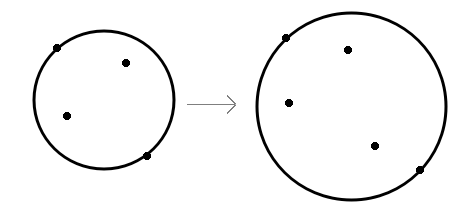
\includegraphics[scale=1]{imgs/welzl}
	\caption{Welzl algoritmo supaprastinimas.}
	\label{imgs:welzl}
\end{figure}
Tačiau apskritimo radimas yra jautrus segmentavimo metu atsiradusiam triukšmui: jeigu po kamuolio segmentacijos fone dar lieka pašalinių objektų, panašių į apskritimą, jie gali būti aptinkami algoritmo vietoje kamuolio. Todėl būtina prieš tai atsirinkti didžiausią regioną, ant kurio bus vykdomas algoritmas - mažai tikėtina, kad triuškmas galėtų sugeneruoti objektą, didesnį už kamuolį.
Kontūrai vėliau užpildomi, rezultate gaunant visą plotą, kuriame yra kamuolys, net jei jis ir uždengtas kitų objektų. \ref{imgs:kamuol} paveikslėlyje matyti, jog kontūrai - vientisas apskritimas, nepaisant to, jog didelę kamuolio dalį dengia ranka.
\begin{figure}[H]
	\centering
	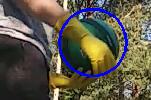
\includegraphics[scale=1]{imgs/kamuol}
	\caption{Kamuolio kontūrai.}
	\label{imgs:kamuol}
\end{figure}
\section{Objektų ir jų padėties atpažinimo algoritmas}
Čia aprašomas objektų padėties atpažinimas bei apibendrintas algoritmas, kaip iš vaizdo gaunama reikiama informacija apie tai, ar kamuolys rankose bei  atliktas žingsnis.
\subsection{Rankos, kamuolio, pėdų  atpažinimas ir tarpusavio sąryšiai}
Atlikus segmentavimą, morfologines transformacijas bei kontūrų užpildymą, turima pakankamai informacijos teiginių apie objektų tarpusavio sąryšius konstravimui.
OpenCV visus paveikslėlius galima reprezentuoti loginėmis matricomis. Tad ranka, kamuolys bei pėdos saugomi kaip loginės matricos, kas įgalina efektyviai atlikti logines operacijas.
\subsection{Kamuolio laikymo ir žingsniavimo atpažinimo algoritmas}
Aukščiau aprašytas procedūras galima apibendrintai aprašyti algoritmu, kuriuo vadovaujasi ir sukurta programinė įranga.
\begin{enumerate}
	\item Vaizdo medžiaga išskiriama į kadrus.  
	\item Kiekvienam kadrui vykdoma segmentacija pagal iš anksto numatytas spalvas, gaunami regionai. 
	\item Regionams vykdomos morfologinės, kontūro radimo operacijos.
	\item Kontūrai užpildomi.
	\item Persidengiantys regionai konvertuojami į logines matricas, atliekamos Būlio disjunkcijos.
\end{enumerate}

Disjunkciją atlikus su kamuolio ir rankos matricomis, gaunama nauja matrica, kurioje teigiama reikšmė reiškia tai, jog šioje vietoje ranka ir kamuolys persidengia. Jeigu matricoje teigiamų reikšmių lyginant su visomis reikšmėmis yra daugiau, negu numatytas santykis, kamuolys yra rankoje. Kamuolio buvimo rankoje būsena yra saugoma atminty sulyg kiekvienu kadru.


Žingsnio išgavimo technika šiek tiek skiriasi. Paeksperimentavus su filmuota medžiaga nuspręsta, jog žemės segmentavimas nėra efektyvus: pilkšva aikštelių spalva atsikartoja daug kur - drabužiuose, fone. Vietoje to suskaičiuojamas pėdų kontūrų kiekis. Jeigu pėdos toli viena nuo kitos - kontūrų atitinkamai bus rasta du. Kita vertus, atliekant žingsnio judesį, kojos (žiūrint iš šono) visada persidengs viena su kita. Todėl daroma prielaida, jog kiekvieno žingsnio eigoje pėdos taip pat persidengs.


 Po segmentavimo ir diliacijos persidengiančių pėdų regionai sudaro vientisą aibę, kuri savo ruožtu turi vienintelį kontūrą - išskyrus atvejus, kai dėl prasto apšvietimo po segmentavimo pėdos regione atsiranda trūkių. Šie trūkiai gali sudaryti mažus regionus, nesiribojančius su kitais, kuriuo atveju randami daugiau nei du kontūrai. Tam, kad algoritmas nepraleistų žingsnio, kontūrai, kurių apimamas plotas mažesnis už tam tikrą reikšmę, yra ignoruojami. Jei vaizdo apdorojimo eigoje aptinkama, jog pėdų segmentų skaičius iš dviejų tapo vienu, nusprendžiama, jog buvo padarytas žingsnis. 

\section{Taisyklės pažeidimo atpažinimas}
Šiame darbe nagrinėjama taisyklė yra oficialiame NBA puslapyje aprašytos 10 taisyklės 13 skyriuje \cite{NBARules}. Taisyklė sako, jog gavęs kamuolį, žaidėjas gali padaryti daugiausiai du žingsnius prieš kamuolį išmesdamas ar atiduodamas kitam žaidėjui. Veiksmų, ją pažeidžiančių, aibė yra didelė - ranką pakišant po kamuoliu (\textit{angl.} carrying), varymasis jau prieš tai suėmus kamuolį (\textit{angl.} double dribble), neteisėtas pėdos (\textit {angl.} pivot foot) pakėlimas ir t.t.. Darbe fokusuojamasi į tą veiksmų poaibį, kuriame žaidėjas žingsniuoja, rankose laikydamas kamuolį. 

Tad taisyklė laikoma pažeista, jeigu tenkinama ši sąlyga:  tuo metu, kol kamuolys laikomas rankose, užfiksuojami daugiau negu du žingsniai. Programa saugo atliktų žingsnių kiekį ir būseną, kada kamuolys yra laikomas rankose, tad tai, jog žaidėjas žingsnius padėjo tame laiko intervale leidžia daryti išvadą, jog kamuolio mušinėjimo veiksmas yra sustabdytas - kitaip vargu, ar žaidėjas būtų spėjęs padaryti daugiau nei du žingsnius. 

Tegu $t_S$- laiko momentas, žymintis žingsnio įvykį $S$. Intervalas $({t_R}_1,{ t_R}_2)$ nusako laiko intervalą, kai kamuolys buvo laikomas rankuose, $R_1$ - kamuolio suėmimas, $R_2$ - kamuolio paleidimas. Tuomet sąlygą, tenkinančią taisyklės pažeidimą, galima aprašyti taip: 

\begin{equation}\label{eq:zingsniai}
\exists {t_S}_1\exists {t_S}_2 \exists {t_S}_3 ( \{{t_S}_1,  {t_S}_2,  {t_S}_3\} \in	({t_R}_1, {t_R}_2) ).
\end{equation}

Ši žingsnių atpažinimo metodika turi svarbų trūkumą - jei žingsniavimo procese kamuolys nors viename kadre išeina iš rankų, intervalas nutrūksta ir žingsniai pradedami skaičiuoti iš naujo. Turint omeny tai, jog rankos ir kamuolio sąlyčio taškų kiekis gali būti itin mažas (priklausomai nuo to, kaip laikomas yra kamuolys bei nuo to, kiek sėkminga buvo segmentacija),tikimybė, jog kamuolys nebus aptiktas rankose, net ir tada, kai jis ten yra, yra reikšminga. Nutrūkus laikymo rankose intervalui, atitinkamai mažėja ir visos $({t_R}_1,{ t_R}_2)$ aibės - tuomet sumažėja ir tikimybė, jog sąlyga \ref{eq:zingsniai} bus tenkinama, galimai padidėjant ir klaidingai neigiamų rezultatų skaičiui.


Siekiant išvengti tokių trukdžių, nuspręsta naudoti skaitiklio principą: saugomas dar vienas kintamasis - skaitiklis, kuris, išėjus kamuoliui iš rankų ribų, mažinamas, ir tik pasiekus reikšmę 0 laikoma, kad kamuolys nebėra rankose. Taip pasiekiamas laikymo rankose intervalo stabilumas - menki skaičiavimo trikdžiai nebesuskaido intervalo, ir jeigu kamuolys tikrai nebėra rankose - programa tą atpažins jau po kelių kadrų ir žingsnius pradės skaičiuoti iš naujo. Tiesa, didžiausia skaitiklio galima reikšmė turi būti pakankamai maža, kad žingsnis nebūtų užregistruojamas jau kamuoliui nebesant rankose. 

\section{Atlikti bandymai ir atvejų analizė}
Šiame skyriuje aprašomas vaizdo medžiagos rinkimas, sukurtos programos išbandymas bei plačiau nagrinėjami atvejai, kuriuose algoritmas neteisingai suklasifikavo duotąją vaizdo medžiagą. 
\subsection{Atlikti bandymai}
Su Xiaomi Redmi 5 Plus kamera skirtingais dienos laikais, iš skirtingų kampų buvo nufilmuoti 5 vaizdo įrašai, kurie vėliau suskarpyti į 5 sekundžių fragmentus. Kiekvienamame vaizdo įrašo fragmente žingsnių taisyklės pažeidimas arba įvyksta, arba ne. Atliekant sukurtos programos bandymus su nufilmuota vaizdo medžiaga pastebėtos kelios problemos: šešėlyje filmuota medžiaga yra netinkama, nes dėl prastos kameros kokybės susilieja fonas ir kamuolys bei pirštinės - visų objektų sodrumas nukrypsta į pilką ir tuomet sunku atskirti skirtingo atspalvio spalvas (kita vertus, gerame apšvietime fonas nebuvo tokia didelė problema, nei tikėtasi - segmentacijos metu buvo puikiai susidorota su skirtumais tarp žalio kamuolio ir medžių). Lygiai taip pat spalvos atpažinimą pasunkina ir žaidėjo nuotolis nuo kameros - prisotinimas, kaip ir filmuojant šešėlyje, nukrypsta į pilką. 


Taip pat iškilo keletas pasirinktų metodikų trūkumų: programa turi sunkumų atpažįstant žingsniavimą, jei žaidėjas filmuotas iš priekio - taip yra dėl pasirinkto aukščiau aprašyto žingsnių atpažinimo būdo, kai žingsnis atpažįstamas tik tada, kai pėdos (sportbačiai) persidengia viena su kita. Atlikus kokį nors sudėtingesnį judesį - tarkim, pasisukimą - programa taip pat linkusi neteisingai tai atpažinti kaip žingsnių taisyklės pažeidimą, kadangi kamuolys užsilieka rankose, o pėdos persidengia bent kelis kartus. 


Siekiant pagerinti problemas su spalvų neatpažinimu buvo stengiamasi kiek įmanoma labiau praplėsti HSV reikšmių intervalą. Bandymo metodais nustatyta, kad batams dėl jų ryškumo ir spalvos unikalumo reikšmių intervalą reikėjo plėsti mažiausiai, o štai kamuolio - daugiausiai (šviesumas nuo 40 iki 200). Pasirinkus per dideles reikšmes klaidingai aptinkamas taisyklės pažeidimas - pavyzdžiui, po rankos segmentacijos lieka ir medžiai, tuomet algoritmas kamuolio ir medžių sąlytį atpažįsta kaip laikymą rankose.


Programai buvo pateikti 22 vaizdo įrašai, iš jų - pusėje įvyksta žingsnių taisyklės pažeidimas, pusėje - ne. Teisingai buvo atrasti 8 taisyklių pažeidimai iš 11 (72.7\% tikslumas) bei 10-yje įrašų iš 11 taisyklės pažeidimo nerasta (90.9\% tikslumas). 2 pažeidimai liko nepastebėti, ir vienas įrašas klaidingai atpažintas kaip turintis pažeidimą. 


\subsection{Klaidingai suklasifikuotų atvejų analizė}

\begin{table}[H]\footnotesize
	\centering
	\caption{Klaidingai suklasifikuoti atvejai}
	\begin{tabular}{|p{2cm}|p{3cm}|p{2cm}|p{2cm}|p{6cm}|}  \hline
		\textbf{Atvejo nr.} & \textbf{Atvejo aprašas} & \textbf{Gautas rezultatas} &     \textbf{Tikėtasis rezultatas} & \textbf{Klaidos paaiškinimas} \\
		
		\hline
		Pirmasis atvejis    & Žaidėjas mušinėja kamuolį stovėdamas, nežymiai kilnoja pėdas, jos arti viena kitos.                & Taisyklė pažeista   & Taisyklė nepažeista & Vaizdo atpažinimo algoritmo trūkumas. Pėdos arti viena kitos - segmentacija išskyrė du beveik besiliečiančius regionus, ko pasekoje rastų kontūrų skaičius periodiškai kas kelis kadrus varijavo tarp vieno ir dviejų. Algoritmas neteisingai tai atpažino kaip žingsnius.                                                                                                                                                                                                                      \\ \hline
		Antrasis atvejis    & Žaidėjas sumuša kamuolį ir jį nusineša už kadro.                                                   & Taisyklė nepažeista & Taisyklė pažeista   & Vaizdo atpažinimo algoritmo ir filmuotos medžiagos trūkumai. Taisyklės pažeidimas neaptiktas dėl dviejų priežasčių. Pirmoji - dėl apšvietimo batų segmentavimas sukūrė atskirtus vienas nuo kito smulkius regionus. Tie regionai tuomet buvo interpretuojami kaip atskiri smulkūs kontūrai, ko pasekoje algoritmas neatpažino padaryto žingsnio. Antroji priežastis - žaidėjo ranka išėjo iš kadro greičiau, nei programa užfiksavo padarytą žingsnį. \\ \hline
		Trečiasis atvejis   & Žaidėjas sumuša kamuolį, paeina kelis žingsnius su kamuoliu rankose, ir tęsia kamuolio mušinėjimą. & Taisyklė nepažeista & Taisyklė pažeista   & Vaizdo atpažinimo algoritmo trūkumas. Darant žingsnį, po segmentacijos kairysis žaidėjo bato aptikta tik maža dalis, nes žaidėjas buvo ganėtinai toli ir šešėlyje, tad batų regionai nesusiliejo į vieną.                                                                                                                                                                                                                                                                                     \\ \hline
		Ketvirtasis atvejis & Žaidėjas įeina į kadrą nešdamasis kamuolį užantyje.                                                & Taisyklė nepažeista & Taisyklė pažeista   & Nei kamuolio, nei jo laikančios rankos nesimatė, tad apie jų poziciją programa nesugebėjo gauti informacijos.                                                                                                                                                                                                                                                                                                                                                                                   \\ \hline
	\end{tabular}
	\label{tab:table example}
\end{table}

Kaip matyti, antruoju ir trečiuoju atveju neteisingą atpažinimą lėmė prastas apšvietimas ir vaizdo kokybė. Segmentacija nesugeba susidoroti su stipriai kintančiu šviesos spektru. Pirmasis atvejis - loginė algoritmo klaida, kadangi nežymūs kojų judesiai buvo palaikyti kaip žingsniai. Ketvirtasis atvejis - per sudėtingas tinkamai atpažinti šiame darbe aprašytomis metodikomis, kadangi remiamasi prielaida, jog kamuolys ir ranka visada matomi.

Panagrinėjus antrąjį atvejį, problemą nuspręsta spręsti euristiškai: vykdant žingsnio atpažinimo algoritmą atmesti kontūrus, kurių apimamas plotas yra mažesnis už tam tikrą slenkstinę reikšmę. 

\subsection{Kiti atvejai}
Tarp vaizdo medžiagos buvo keli įrašai - ribiniai atvejai, kuriuose sunku pasakyti, ar žaidėjas pažeidė taisyklę ar ne. Vienas iš vaizdo įrašų žaidėjas sumuša kamuolį, prieš jį suemant padaro vieną žingsnį (NBA terminologijoje tai vadinasi \textit{gather step}), tuomet kamuolį pilnai suema ir padėjęs du žingsnius išeina už kadro. Tokio tipo dvižingsnis dažnai pagauna teisėjų ir žiūrovų dėmesį, tačiau realiu laiku dažnai sunku pasakyti, ar taisyklė pažeista, ar ne - nors pagal . Vaizdo medžiagą parodžius trim žmonėm du iš jų pareiškė, jog žingsnių taisyklė pažeista. Programa, apdorojusi vaizdo medžiagą sugebėjo teisingai nuspręsti, jog taisyklė nėra pažeista. Kitas atvejis - vaizdo įraše atliekamas judesys, vadinamas „eurožingsniu“ (\textit{angl.} eurostep), tačiau padedant vieną papildomą žingsnį. Judesys atliktas greitai, dėl to realiu laiku stebėtojui gali būti sunku nustatyti, ar taisyklė pažeista. Programa teisingai atpažino šį ribinį atvejį kaip pažeidžiantį taisyklę. 


\sectionnonum{Rezultatai ir išvados}
Šiame darbe buvo atlikta kompiuterinės regos metodų analizė, Python programavimo kalba įgyvendintas žingsnių taisyklės pažeidimo algoritmas, kuris buvo išbandytas realia vaizdo medžiaga. 
Vaizdo medžiagą, kurioje pažeista taisyklė, programa suklasifikavo 72.7\% tikslumu. Vaizdo medžiagą, kurioje nėra pažeista taisyklė, programa suklasifikavo 90.9\% tikslumu. Didžiausias taisyklės atpažinimo klaidų šaltinis - prastas apšvietimas, dėl ko stipriai kinta objektų atspalviai, šviesumas ir sodrumas, ko pasekoje segmentacija pagal spalvą nesugeba atpažinti objektų, kurių atspalvio, šviesumo ir sodrumo intervalai yra nustatyti iš anksto, nekintantys. Objektų atpažinimas pagal spalvą yra labai jautrus išoriniams faktoriams, tad tolimesniuose darbuose rekomenduojama patyrinėti kitus metodus. Taip pat siekiant geresnių rezultatų siūloma išgauti kuo geresnės kokybės vaizdo medžiagą.
Nepaisant to, programa puikiai susidorojo su atvejais, kuriuose apšvietimas yra geras, net ir tais, kuriuose pažeidimą pamatyti plika akimi sudėtinga. 


\printbibliography[heading=bibintoc]  % Šaltinių sąraše nurodoma panaudota
% literatūra, kitokie šaltiniai. Abėcėlės tvarka išdėstomi darbe panaudotų
% (cituotų, perfrazuotų ar bent paminėtų) mokslo leidinių, kitokių publikacijų
% bibliografiniai aprašai.  Šaltinių sąrašas spausdinamas iš naujo puslapio.
% Aprašai pateikiami netransliteruoti. Šaltinių sąraše negali būti tokių
% šaltinių, kurie nebuvo paminėti tekste.

\appendix  % Priedai
\section{Nuoroda į GitHub}
\url{https://github.com/LukasCed/basketball-rule-violation-recognition}

\end{document}
